\documentclass[10pt,twocolumn,letterpaper]{article}

\usepackage{cvpr}
\usepackage{times}
\usepackage{epsfig}
\usepackage{graphicx}
\usepackage{amsmath}
\usepackage{amssymb}
\usepackage{algorithm}
\usepackage[noend]{algpseudocode}


\makeatletter
\def\BState{\State\hskip-\ALG@thistlm}
\makeatother

% Include other packages here, before hyperref.

% If you comment hyperref and then uncomment it, you should delete
% egpaper.aux before re-running latex.  (Or just hit 'q' on the first latex
% run, let it finish, and you should be clear).
\usepackage[breaklinks=true,bookmarks=false]{hyperref}

\cvprfinalcopy % *** Uncomment this line for the final submission

\def\cvprPaperID{****} % *** Enter the CVPR Paper ID here
\def\httilde{\mbox{\tt\raisebox{-.5ex}{\symbol{126}}}}

% Pages are numbered in submission mode, and unnumbered in camera-ready
%\ifcvprfinal\pagestyle{empty}\fi
\setcounter{page}{4321}
\begin{document}

%%%%%%%%% TITLE
\title{Dynamic object detection and reconstruction using multi-view bootstrapping}


\maketitle
%\thispagestyle{empty}

%%%%%%%%% ABSTRACT
\begin{abstract}
Reconstruction of dynamic scenes from multiple unsynchronized cameras in the wild is a challenging problem. Most of the research in the multi camera based reconstruction has been focused in two aspects. With multiple cameras being stationary with dynamic objects in the scene or static scene with cameras moving. We propose a algorithm to solve the problem of dynamic scene reconstruction from multiple moving cameras. We also show the advantages of our method by proposing a improvement in detection using multi-view bootstrapping. We use semantic keypoints and spatio-temporal bundle adjustment to densily reconstruct the dynamic scenes. Using the accurate reconstructions, we improve the accuracy of the keypoint detections. The novel method of using multiple camera based method for training the detections can be applied to any task in computer vision.      
%Multi camera based understanding of dynamic scenes from unsynchronized images is a challening problem in reconstruction. We propose a solution to the problem of 3D reconstruction of multiple moving rigid objects from unsynchronized multiple cameras. Most of the reconstruction piplines leverage reconstruction using reprojection error of features, we propose a novel semantic features pipeline and object based feature tracking for reconstruction of dynamic objects. We leverage multiple rigid object constraints in a bundle adjustment framework to improve the reconstuction. 
\end{abstract}
%sdsd
\section{INTRODUCTION}
Reconstruction and infering about a scene is the most important problem in computer vision. Although there have been plethora of work in scene understanding and reconstruction from images and videos. Most of the methods cannot completely infer the dynamics of a scene because of bottleneck of the number of views. We believe this problem can be solved using multiple cameras recording the scene. Most of the research in this direction has been from multiple static cameras. We propose reconstruction of dynamic objects captured from multiple unsynchronized cameras. We believe accurate reconstruction of scene in the wild can be used for training wide range of computer vision tasks like detection, semantic segmentation etc. Further reconstructions from multi camera systems have wide applications in areas like robot navigation, virtual reality and Autonomous driving. 

With the advent of deep learning most of the research has focused on end-to-end learning of most of the tasks in computer vision. We believe that geometric constraints impose a very strong prior on the scene and exploiting these constraints help in learning the reconstruction of a scene. Our method proposes a reconstruction pipeline using features from the deep learning based keypoint detection algorithm. We further use geometry based multi-view constraint to improve the detection accuracy in the images. We show results on keypoint based improvement algorithm but the multi view information can be used to improve and learn any vision task like detection segmentation etc.

Dynamic objects reconstruction is a well studied problem due to its applications in all the computer vision problems. Most of the earlier works have used sparse features to segment and reconstruct moving and stationary objects simultaneously. We interpolate the idea to semantic keypoints i.e. wheels, head lights etc and densely reconstruct the enviroment. We add multiple constraints using bundle adjustment like motion prior, semantic cues for improving the reconstructions.

The main contributions of the paper are outlined:
\begin{enumerate}
%\item Novel instance keypoint detection pipeline for reconstruction of moving objects.
\item  Time synchronization of multiple videos by optimizing for motion of moving objects. 
\item Constraint Bundle adjustment for reconstruction of dynamic moving objects viewed from multiple cameras. 
\item Improving the detection accuracy using reconstruction of dynamic scenes in the wild.
\end{enumerate}

\section{RELATED WORK}
\subsection{Multi-Camera systems}
%Multiple methods have been proposed to solve the problem of reconstruction from multiple camera sensors. 
\subsection{3D reconstruction}

\subsection{Geometry for learning}
%Multiple methods have been proposed to use geometric constraints to improve the learning.
\section{METHOD}
We follow the template version of 3D reconstruction from multiple cameras i.e. feature detection and tracking, correspodence of the keypoint across views and then bundle adjustment for accurate reconstruction of the 3d points. In each of the segments of the pipeline we incorporate geometric and semantic information of the objects for better reconstruction. We propose instance keypoint segmentation for better feature detection of important points on the objects. 
We first formulate the problem statement. Lets assume $N$ video cameras observing $M$ moving object with $P$ 3d points over time $X^p(t)$ and their 2D projection $x^p_n(f)$ on camera $p$ and frame $f$ is given as:

\begin{align*}
 \begin{bmatrix} x_n^p(f) \\ 1  \end{bmatrix} = K_n(f)[R_n(f) | T_n(f)] \begin{bmatrix} X_n(f) \\ 1  \end{bmatrix}
\end{align*} 

where $K_n(f)$ is the intrisic camera matrix, $R_n(f)$ and $T_n(f)$ are the relative camera rotation and translation, respectively. We denote this transformations $x_c^n(f) = P_n(f,X^n(t))$
%-------------------------------------------------------------------------

\subsection{Time synchronization from multiple videos}
All the videos captured are taken from unsynchronized cameras. The first problem is to solve the synchronization problem by observing motion of onjects from multiple views. we propose a multi camera video synchronization method for reconstructing from multiple videos. We assume that the rotation and translation of the object to be constant over time. We follow the work of \cite{gaspar2014synchronization}, which synchronizes the time offset between two video frames assuming motion of a rigid object from non overlapping views. We extend the formulation further to synchronize multiple videos observing a moving rigid objects. The error to be minimized for synchronization is:
\begin{equation}
  	E_s(\delta) = min \ E_{R}(\delta,q) + E_{T}(\delta,T,q) + (q^{T} q -1)^2
\end{equation}
where $\delta$ is the time offset of each video with respect to the global time. where $E_R(\delta,q)$ gives the error in rotation with respect to the offset for the moving object and $E_T(\delta,T,q)$ gives the error in translation with respect to the offset. q and T are the translation and rotation in quaternion respectively.


\subsection{Multi-view Object Fitting}
We currently have tracks of objects and thier respective keypoints in each individual video for all videos of the scene. For accurate reconstruction of objects from multiple views we need to find corrospondences across views. We propose a object specific bundle adjustment for finding correspondes across views. Lets assume we have $h$ object proposals in $N$ videos at any time instant $t$. The problem of correspondence is finding $g$, where $g \subset h$ object bounding boxes which belong to the same object. Since there is a spatial constraint on the bounding boxes over multiple views, Fig \ref{fig:corr} shows the bundle adjustment we use to find correspondes across views. We propose a ransac based methodology for finding correspondenses across views and minimize the following reprojection error:

\begin{equation}
  	E_r =\sum_{n=1}^{N} \sum_{p=1}^P \sum_{f=1}^{F_n} V_n^p(f) ||P_n(f,X^p(t)) - x_n^p(f)||^2
\end{equation}
   
where $E_r$ is the image reprojection error, $V_n^p(f)$ is a binary indicator of the visibilty of the keypoint. We add additional constraints like symmetry and the length of different joints of the object for accurate fitting of the rigid object in 3D. A joint in 3d can be defined as the difference of the 3D points between the centers of the joint. We define a joint as $J(p1,p2) = X^{p1}(t) - X^{p2}(t) $ where p1 and p2 correspond to different parts of the rigid object which are linked. 

\begin{equation}
  	E_l = \sum_{r=1}^R ||J(r) - E(J(r))||^2  
\end{equation}

where $E(J(r))$ is the mean length of joint $r$. We model the symmetry constraint in the budle adjustment for better reconstruction of rigid objects.
\begin{equation}
  	E_j = \sum_{q = 1}^Q ||J(q) - J(S(q))||^2
\end{equation}

where $S(q)$gives the corresponding symmetric joint of $q$ i.e. if q is the joint connecting the left wheels of a car S(q)is the joint connecting the right wheels of the car.


\begin{algorithm}
\caption{Multi-view Object Correspondence}\label{euclid}
\begin{algorithmic}[1]
%\Procedure{MyProcedure}{}
\State $\textit{n} \gets \text{Total object Hypothesis }$
\State $s \gets 0$
\BState \emph{top}:
\If {$i > \textit{stringlen}$} \Return false
\EndIf
\State $j \gets \textit{patlen}$
\BState \emph{loop}:
\If {$\textit{string}(i) = \textit{path}(j)$}
\State $j \gets j-1$.
\State $i \gets i-1$.
\State \textbf{goto} \emph{loop}.
\State \textbf{close};
\EndIf
\State $i \gets i+\max(\textit{delta}_1(\textit{string}(i)),\textit{delta}_2(j))$.
\State \textbf{goto} \emph{top}.
%\EndProcedure
\end{algorithmic}
\end{algorithm}

\subsection{Spatio-Temporal Bundle Adjustment}
Once we have the correspondences across cameras and views, We get the fit a motion model based rigid object over time. The formulation is given by:

\begin{equation}
 E = arg \underset{X(t),\{K,R,t\},\alpha,\delta} {\mathrm{min}} \sum_{t=1}^T E_r +  E_j +  E_l +  E_m + E_s
\end{equation}

where $w$ represents the weights of each term in the bundle adjustment. $E_m$ is defined as the motion prior over the trajectory of the points.

\begin{equation}
E_m = \sum_{p =1 }^P \sum_{i = 1}^{T^n -1} ||\frac{X^p(t^{i+1}) - X^p(t^{i})}{t^{i+1} - t^{i}}||^2 (t^{i+1} - t^{i})
\end{equation}
\begin{figure}
  \centering
    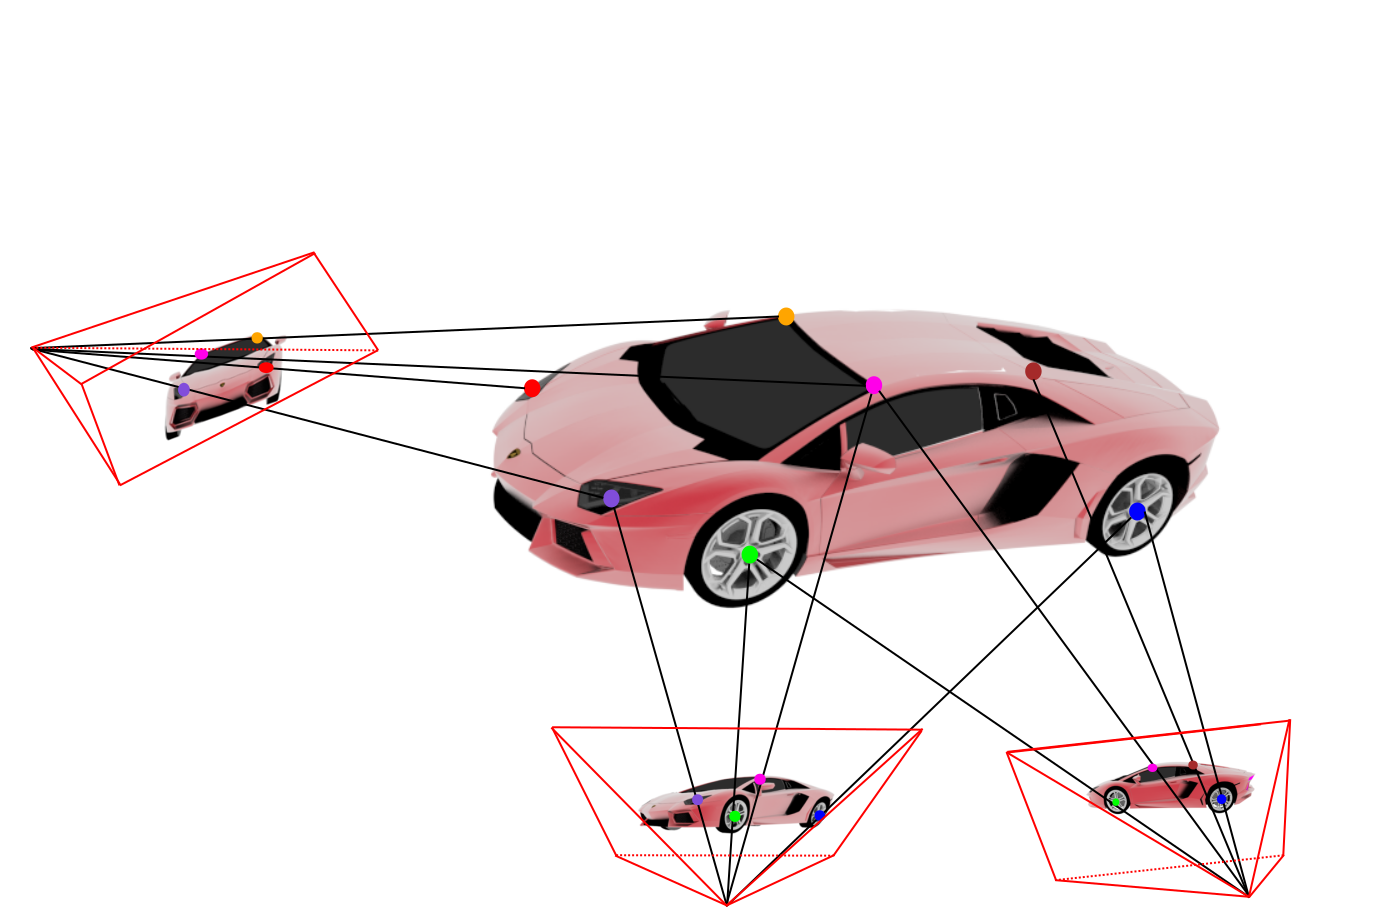
\includegraphics[width=0.4\textwidth]{images/corr}
  \caption{The picture depicts the projection of 3D keypoints of car onto thier respective videos}
  \label{fig:corr}
\end{figure}

\subsection{Local features based Refinement}
Although the reocnstructions from the constrained bundle adjustment works well. It is highly dependent on the keypoint detector. We propose to improve the reconstruction by using local features like sift around the keypoints. Since the motion of the object is stationary 
\subsection{Finetune Network}
We 
\section{Implementation Details}

\subsection{Instance Aware Keypoint detection}
Given a images with multiple moving objects. The amount of objects which can move can be sorted into a small set of categories like cars and humans. We propose a instance keypoint detection on these categories for improving the reconstruction of these objects. We leverage deep learning framwork for fast and accurate detection of semantic features in images. We pass the input image through a detection pipeline and each detected bounding box is passed through a object specific keypoint detection pipeline for computation of semantic features in an image.  

\subsection{Object aware keypoint tracking}
Tracking of keypoints has generally been considered as a search problem over the image space for features of similar shape in adjustcent images. Semantic aware tracking correspondences to tracking of the important parts using the knowledge of the object i.e. the keypoints on the wheels are tracked by finding the correspondences of cars overtime. This gives a better tracks of the keypoints and longer correpondeces compared to the feature based tracking methods. 

{\small
\bibliographystyle{ieee}
\bibliography{egbib}
}
\end{document}
